\documentclass[border=6pt]{standalone}
\usepackage{tikz}
\usetikzlibrary{arrows.meta,positioning,calc,shapes.geometric,fit,backgrounds,patterns,matrix,decorations.pathreplacing}
\begin{document}
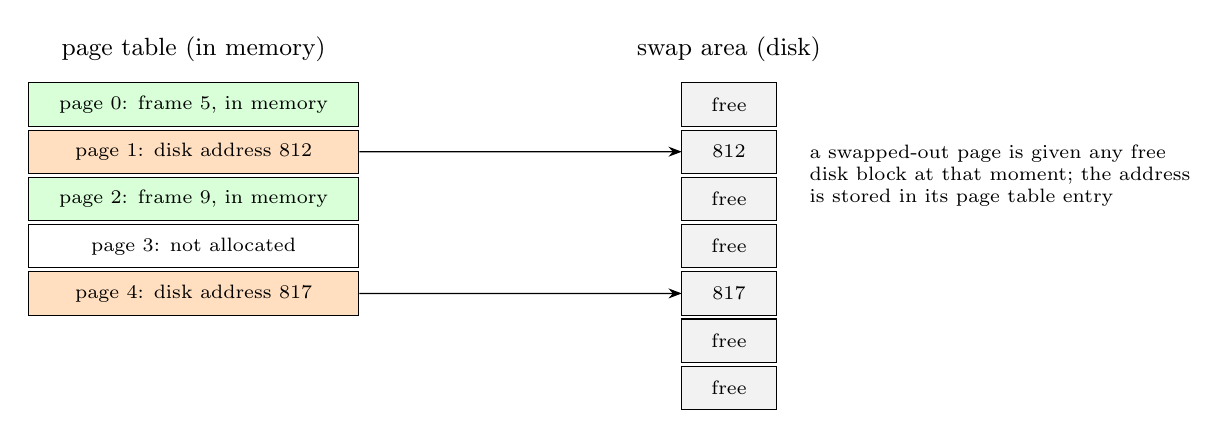
\begin{tikzpicture}[>=Stealth,font=\small]
\tikzstyle{b}=[draw,minimum height=0.55cm,font=\scriptsize]
\node[font=\small] at (1.8,2.1) {page table (in memory)};
\foreach \i/\t/\c in {0/{page 0: frame 5, in memory}/green!15,1/{page 1: disk address 812}/orange!25,2/{page 2: frame 9, in memory}/green!15,3/{page 3: not allocated}/white,4/{page 4: disk address 817}/orange!25} \node[b,minimum width=4.2cm,fill=\c] (p\i) at (1.8,1.4-\i*0.6) {\t};
\node[font=\small] at (8.6,2.1) {swap area (disk)};
\foreach \i in {0,...,6} \node[b,minimum width=1.2cm,fill=gray!10] at (8.6,1.4-\i*0.6) {\ifnum\i=1 812\else\ifnum\i=4 817\else free\fi\fi};
\draw[->] (p1.east) -- (8.0,0.8); \draw[->] (p4.east) -- (8.0,-1.0);
\node[font=\scriptsize,align=left,anchor=west] at (9.5,0.5) {a swapped-out page is given any free\\ disk block at that moment; the address\\ is stored in its page table entry};
\end{tikzpicture}
\end{document}
